\documentclass[11pt]{article}
\usepackage{../stat110}
\usepackage{graphicx}

%\STAFF

\begin{document}
\SectionNotes{1}{Counting}{Luis Perez (luisperez@college.harvard.edu)}{Aidi Zhang(aidizhang@college.harvard.edu)}

\section*{General Course Notes}
\subsection*{Welcome to Stat 110!}
This is a difficult but highly rewarding class designed to make you a better thinker. Do you best to \textbf{keep up} with the concepts -- the material is \textit{cumulative}. If you feel like you're falling behind or having even just a bit of trouble, make use of our resources:
\begin{itemize}
\item Statistics 110 Textbook (\href{http://www.amazon.com/gp/product/1466575573/ref=as_li_tl?ie=UTF8&camp=1789&creative=390957&creativeASIN=1466575573&linkCode=as2}{buy})
\item Past homeworks, midterms, section problems
\item Current section problems
\item 2011's Full Class (\href{http://projects.iq.harvard.edu/stat110/about}{stat110.net})
\item Joe and your TFs.
\end{itemize}
\subsection*{Where to find us, how to reach us.}
E-mail: luisperez@college.harvard.edu \\
Phone: (936) - 250 - 0347 \\
Section: Tuesday 12:00 PM - 1:00 PM in SC 706 \\
Office Hours: Wednesday 10:00 PM - 12:00 AM (Quincy D-Hall) \\

E-mail: aidizhang@college.harvard.edu \\
Phone: (617) - 637 - 5532 \\
Section: Wednesday 4:00 PM - 5:00 PM in SC 304\\
Office Hours: Wednesday 8:00 PM - 10:00 PM (Quincy D-Hall) \\

\section*{Combinatoric (Counting) Overview, General Class Advice}
Combinatorics is a really cool subject. In a sense, you're learning how to count the `right' way (ie, in a way that lets you generalize to quantities too large to count normally). One cool (though most students find tricky) part of combinatorics is that there are almost always multiple ways to find an answer. However, not all ways are created equal. There are usually a few fas, easy, ways to go about `counting'. The only way I know to pick up an intuition for which way to `do it' is to practice -- the more problems you expose yourself to, the better you'll get at trying the right approach on the first try. \\

Combinatorics is a foundational part of statistics. This is a class about $\textbf{learning how to think}$ (and we're starting with learning how to count), not messy summation, integrals, etc. In this class, if you find messy notation in your work, you might not be approaching the problem the elegant way. There's often a neat way to do the problem that's self-annotating, or very easy to check your work on. At the very least, if something is getting messy, take a few minutes to re-think your approach, to chat with friends, TFs, or even Professor Blitzstein. \\

\section*{Frequently Asked Questions\footnote{Note that a simple Google Search, given the popularity of this class, will lead to almost surely complete to any question.}}

\begin{description}
\item[Should I take this class?] No, unless you want to be an awesome person, then yes.
\item[What are some tips in doing well?] Read the textbook, come to section, come to lecture, in that order.
\item[What kind of math background do I need?] Being comfortable with discrete math helps, but you can also learn it along the way. The ability to reason logically is the most helpful part from a mathematics education.
\item[More questions?] - \texttt{Email us or post on Quora!}
\end{description}

\section*{Useful Mathematical Facts}
\begin{align*}
n! = 1 \cdot 2 \cdot 3\cdots n \tag{0! = 1} \\
{n \choose k} = \frac{n!}{k!(n-k)!} = \frac{n(n-1)...(n-k+1)}{k!}\\
{n \choose k} = {n \choose n-k} \\
\end{align*}

\section*{Counting (a.k.a Combinatorics)}
\begin{description}
	\item[Multiplication Rule] - This is pretty straight forward, and for the visual learners, essentially falls from writing out all the possibilities in a systematic way. Suppose you flip a coin twice. How many possible outcomes are there? For both flips, the event belongs to the set $\{H,T\}$, so there are 2 possible outcomes on each flip. Each of the first outcomes from the first flip branches into two possible outcomes. In total, we have $2 \cdot 2$ outocomes of the form $\{HH, HT, TH, TT\}$.

More generally, if have a compound experiment (an experiment with multiple components). If the 1st component has $n_1$ possible outcomes, the 2nd component has $n_2$ possible outcomes, and the $r$th component has $n_r$ possible outcomes, then overall there are $n_1n_2 \dots n_r$ possibilities for the whole experiment.

\textbf{Another Example} There are 17 freshman dorms and 12 upperclassmen houses at Harvard, which means that there are a total of $(17 + 12) \cdot 17 \cdot 12 = 5916$ combinations of dorms that a Harvard student can be assigned to, assuming every student attended Visitas, lived on campus freshman year, and lived on campus at least two years.
	\item[Sampling Table] - The sampling tables describes the different ways to take a sample of size $k$ out of a population of size $n$.\\
		\begin{table}[htb!]
		\begin{center}
	    	    \setlength{\extrarowheight}{1pt}
			\begin{tabular}{r|cc}
				 & \textbf{Order Does Matter}~~ & \textbf{Order Doesn't Matter} \\ \hline
				\textbf{With Replacement}~~~ & $\displaystyle n^k$~~~~~~~~~~~~~~ & $\displaystyle{n+k-1 \choose k}$~~~~~ \\
				\textbf{Without Replacement} & $\displaystyle\frac{n!}{(n - k)!}$ & $\displaystyle{n \choose k}$
			\end{tabular}
		\end{center}
		\end{table}
\end{description}

\section*{Statistics}
\begin{description}
	\item[Experiments/Outcomes] - An experiment generates an outcome from a pre-determined list.
	\item[Sample Space] - The sample space, denoted $S$, is the set of possible outcomes.
	\item[Event] - An event is a subset of the sample space, or a collection of possible outcomes of an experiment. We say that the event has occurred if any of the outcomes in the event have happened.
	\item[Na\"{i}ve Definition of Probability] - \emph{If the likelihood of each outcome is equal}, the probability of any event happening is:
		\[P(\textnormal{Event}) = \frac{\textnormal{number of favorable outcomes}}{\textnormal{number of outcomes}}\]
\end{description}


\begin{comment}
\section*{Story Proofs}
\begin{description}
	\item[Definition] - A proof by interpretation or application rather than by algebra or calculus. Examples of story proofs would be combinatorial proofs, which there are three examples of below, where two quantities are equated as it it shown that they are two ways of counting the same thing.
	\item[Example 1] - Symmetry Rule for Binomial Coefficients
		\[{n \choose k} = {n \choose n-k}\]
		If you want to choose $k$ people out of $n$, you can either directly pick the $k$ people to be included (LHS), or pick the $n-k$ to be not included (RHS).
	\item[Example 2] - Product of ${r \choose m}$ with ${m \choose k}$
		\[{r \choose m}{m \choose k} = {r \choose k}{r-k \choose m-k}\]
		In a class of $r$, you want to pick a team of $m$ members with $k$ leaders. You can either first choose the team (${r \choose m}$ ways) and then the leaders out of the team (${m \choose k}$ ways) (LHS), or you first choose the leaders (${r \choose k}$ ways) and then choose the remaining members out of the remainder of the class (${r-k \choose m-k}$ ways) (RHS).
	\item[Example 3] - Vandermonde Identity
		\[\sum_{i=0}^k {m \choose i}{n \choose k-i} = {m + n \choose k}\]
		A class contains $m$ females and $n$ males. We want to find all of the ways to form teams of $k$ students. We can find the number of teams that include $i$ females - there are ${m \choose i}$ ways to choose the females and ${n \choose k-i}$ ways to choose the males, for a total of ${m \choose i}{n \choose k-i}$ ways to choose a team with $i$ females. We sum over $i$ to get the total number of teams (LHS), which we know is also ${m + n \choose k}$ (RHS).
\end{description}
\begin{exercise}
It is a well known fact that:
\begin{align*}
\sum_{k=0}^{n} { n \choose k } = 2^n
\end{align*}
Practice your story proof skills by giving two ways of counting the same thing that objective
\end{exercise}
\begin{solution}
\end{solution}
\end{comment}

\section*{Practice Problems}
\vskip .2 in

\begin{exercise}
Let $S$ be the sample space corresponding to rolling a die. What are the outcomes? Give an example event. How many possible events are there? Given the naive definition of probability, does $P(S)$ make sense, and if so, what is it?
\end{exercise}
\begin{solution}
The outcomes are $1,2,\cdots,6$, so the sample space is $S = \{1,2,3,4,5,6\}$. An example event is something along the lines of "get an event number", which can be represented as $A  = \{2,4,6\} \subset S$. The total number of possible events corresponds to the number of possible subsets of $S$. For our example, this is given by $2^{6}$. Calculating $P(S)$ makes perfect sense and is simply $P(S) = 1$.
\end{solution}

\begin{exercise}
A friend of yours makes the following claim:
\begin{align*}
\sum_{k=0}^{n} { n \choose k } = 2^n
\end{align*}
Do you have reason to believe him/her? Don't worry about proving this, as we'll learn how in future sections, just see if you can relate it to the previous problem.
\end{exercise}
\begin{solution}
Another way to count the subsets of a set is to count how many sets are of a specific size. For example, there are $6$ sets of size $1$ in the above problem, ${6 \choose 2}$ sets of size $2$, and so on. Given this, we would be inclined to believe the above equation since both sides count the number of subsets of a set of size $n$.
\end{solution}


\begin{exercise}
Let $S$ be the sample space corresponding to the sum of a two dice roles. Write $S$ explicitly. Does the na\"{i}ve definition of probability apply? Why or why not?
\end{exercise}
\begin{solution}
We can write $S$ as $\{2,3,4,5,6,7,8,9,10,11,12\}$. The na\"{i}ve definition of probability does not apply because each event isn't equally likely. For example, there is only one way for the dice to sum to $2 = 1 + 1$, but multiple ways to sum to 4 $4 = 2 + 2$ and $4 = 3 + 1$.
\end{solution}


\begin{exercise}
How many distinct rectangles can one construct such that each of their 4 sides is part of a $10 \times 10$
 grid? (Compliments of Viviana)
\end{exercise}
\begin{solution}
There are multiple ways to think about this problem. One way is to notice that each rectangle is uniquely specified by two distinct vertical and two distinct horizontal lines. We can therefore count the number of rectangles by simply counting the number of ways to choose two distinct vertical lines and two distinct horizontal lines.
$$
{11 \choose 2}{11 \choose 2} = 3025
$$
Another way to think about the problem consists of noting that a rectangle can be specified by pairs of opposite vertexes (there are two pairs per rectangle). Then we can count the number of rectangles by counting the number of ways to choose these vertices.
$$
\frac{121 \times 100}{2} = 6050
$$
However, as mentioned, each rectangles is specified by two distinct pairs, so the total number of rectangles is $\frac{6050}{2} = 3025$.
\end{solution}

\begin{exercise}
How many distinct squares can one construct such that each of their sides is part of a $ N \times N$ grid.
\end{exercise}
\begin{solution}
We can calculate this using a well-known sum by considering the number of squares of each particular area.
$$
\sum_{k=1}^n k^2 = \sum_{k=1}^{n} (n-k+1)^2 = \frac{n(n+1)(2n+1)}{3!}
$$
In this case,
\end{solution}


\section*{It's Magic!}
We will now demonstrate a simple magic trick (drumroll, please.). \\
The trick works as follows. From a standard $52$ card deck, a volunteer from the audience selects $5$ cards and shows the $5$ cards to Aidi. Aidi then proceeds to show $4$ of the $5$ cards to Luis, at which point, Luis will correctly determines the suit and value of the fifth, unseen card.
After having seen the magic trick, let's just do some counting.

\begin{exercise}
How many possible hands could our volunteer have chosen?
\end{exercise}
\begin{solution}
$${52 \choose 5} = 2598960$$
\end{solution}

\begin{exercise}
Let's generalize a bit. Suppose we have a deck with $N$ cards. Aidi must show Luis $4$ of the $5$ cards. Give an argument for why the magic trick won't work for a deck with $N > 124$ cards. \\
Hint: Each card Luis doesn't see has to be uniquely identified by the cards Aidi shows him.
\end{exercise}
\begin{solution}
Luis sees four cards, so the number of unseen cards are $N - 4$. If we assume no cheating, Aidi must use the four cards he shows Luis to uniquely specify each of the $N - 4$ cards. We therefore need to - given five random cards, how many unique ways are there to show $4$ of the $5$ to Luis. First, Aidi must choose $4$ cards to show, and of those cards choose, she can show them in any order to Luis. We have
$$
{5 \choose 4}4! = 120
$$
unique ways to show the cards. If the number of unseen cards exceeds this value, then it is impossible for the trick to work, since there will always exists at least one combination of cards shown by Aidi which correspond to more than one card from the deck, and Luis would be unable to determine the hidden card. Therfore, the magic trick will fail when:
$$
N - 4 > 120 \implies N > 124
$$
as desired.
\end{solution}

\begin{exercise}[Bonus]
How did we do it?
\end{exercise}
\begin{solution}
For 52 cards, there's a simple way to do this. Essentially, first note that from a given set of 5 cards, there will always be two distinct cards from the same suit. Next, note that for two distinct cards from the same suit, the ``distance'' in their values is always $<= 6$ if we ``wrap around'' from 13 to 1 (for those familiar, this would be mod 12 arithmetic with some modifications). For example, the shortest distance from 10 to 2 is 5 since we have $10,11,12,13,A,2$, so it takes five steps to get to $2$ from $10$.

We then just need to encode this information.

What Aidi does, given the $5$ cards, is find the two in the same suit. After finding these two cards, she selects the card to which, when we add a value $1 \leq x \leq 6$, we arrive at the second card using the procedure described above and show that card last (ie, if the card she picks are 10 and 2, she will show the 10 card last and hide the 2). Next, she needs to encode the difference, and she does this using the remaining 3 cards, which can encode a total of $6!$ distinct values. Given any three cards, simply label them $L,M,H$ for the lowest, middle, and highest value card (break ties alphabetically with suits). With this labeling, you can encode six distinct values (LMH, LHM, MLH, MHL, HLM, HML).
\end{solution}

\section*{More Counting!}
\begin{exercise}
Determine the number of ways to traverse a 8 x 10 grid, as shown below, from the bottom left corner to the upper right corner if you are only allowed to move to the right and upwards.

\begin{center}
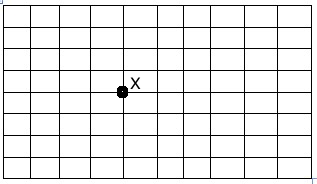
\includegraphics[scale=0.6]{chessboard}
\end{center}

\noindent Extra: How many ways are there if you are required to pass through the point on the grid labeled X?
\end{exercise}
\begin{solution}
There are 16 moves required to move from the bottom left to upper right corner. Out of these 18 moves, 8 must be up moves and 10 must be right moves. Hence, there are $\binom{18}{8} = \binom{18}{10}$ number of possible paths. Note that this is true because of one of the useful mathematical facts mentioned above.\\
\\
Extra: This is simply using multiplication rule on two similar sub-problems. Following the logic above, there are $\binom{8}{4}$ number of paths from bottom-left to X, and $\binom{10}{4}$ number of paths from X to upper-right. Thus, we have $\binom{8}{4} \cdot \binom{10}{4}$ total paths that pass through X.
\end{solution}

\begin{exercise}
For the following questions, consider numbers where digits are only chosen from $D = \{1,2,3,4,5,6,7,8,9\}$, i.e. numbers that can be built without the digit $0$.

\begin{enumerate}
\item How many four-digit numbers are there?

\item How many four-digit numbers have four different digits?

\item How many four-digit numbers have strictly increasing digits?

\item How many four-digit numbers have non-decreasing digits?

\end{enumerate}

\end{exercise}
\begin{solution}
In order:

\begin{enumerate}
\item $9^4$.

\item $9 \cdot 8 \cdot 7 \cdot 6 = 3024$.

\item This is equivalent to choosing a subset of $4$ elements from a set of digits $D = \{1,2,3,4,5,6,7,8,9\}$ without replacement, which is $\binom{9}{4} = 126$ since every set of four elements from $D$ corresponds uniquely to such a four-digit number with strictly increasing digits.

\item This is equivalent to choosing a subset of $4$ elements from a set of digits $D = \{1,2,3,4,5,6,7,8,9\}$ with replacement, which by Bose-Einstein's, is $\binom{9+4-1}{4} = \binom{12}{4} = 495$.\\
\\
If you don't manage to see the above "elegant" method, you can also brute force your way through this, although this is definitely not recommended. Just for the sake of demonstration:\\
\\
We consider cases. In the case where all four digits are unique, there are $\binom{9}{4} = 126$ possibilities as above. In the case where only 2 digits are repeated, there are $3 * \binom{9}{3} = 3 * 84 = 252$. In the case where there are two pairs of 2 digits being repeated, there are $\binom{9}{2} = 36$ possibilities. In the case where there are only 3 digits repeated, there are $2 * \binom{9}{2} = 72$ choices. And finally, in the case where all digits are repeated there are $\binom{9}{1} = 9$ choices. Adding all of the above cases up, we get a total of $126 + 252 + 36 + 72 + 9 = 495$ non-decreasing numbers.
\end{enumerate}
\end{solution}

\begin{exercise}[Homework!]
6 men and 6 women are made to stand in a line. What is the probability that no 5 men are standing consecutively to each other?
\end{exercise}
\begin{solution}
We would want to calculate the complement - which is the probability that the longest length of consecutive men is either 5 or 6 - because the complement is much easier to compute. The number of permutations such that the longest length of consecutive men is 6 is $7! \cdot 6!$ (we view the 6 consecutive men as one entire object, so we're attempting to arrange only $7$ objects. There are $6!$ ways to permute the 6 men in the block amongst themselves).\\
\\
Now, we count the number permutations such that the longest length of consecutive men is exactly $5$. We have $6$ women, $1$ man, and a block of $5$ men. There are $6$ ways to choose the $1$ man. The total number of possible arrangements of this group of 8 objects (we consider the 5 men group a single object) where the $1$ man and $5$ men block are NOT adjacent, is $[8! - 2(7!)]$. We therefore have $6 \cdot 5! \cdot [8! - 2(7!)]$ permutations in this case.\\
\\
Hence, the final answer is:

$$1 - \frac{7! \cdot 6! + 6! \cdot [8! - 2(7!)]}{12!}$$

(Note: this is a pretty involved question that cleverly redefines "objects" to permute. Take your time to think through it!)

\end{solution}

\end{document}

